\section{Silvanet-Technologie}

Das Startup namens \href{https://www.dryad.net/}{Dryad}\footnote{https://www.dryad.net/} mit Sitz in Berlin hat sich zum Ziel gesetzt, die Zahl der Waldbrände zu verringern, indem es sie so schnell wie möglich entdeckt und die Behörden warnt.
Ein Team für die Entwicklung von Hardware und eingebetteten Systemen beschäftigt sich mit der Entwicklung kleiner solarbetriebener Sensoren, die Veränderungen in der Zusammensetzung der Umgebungsluft erkennen können.
Wenn eine Veränderung festgestellt wird, wird ein Scan initiiert und eine eingebaute künstliche Intelligenz bestimmt, ob es sich um die Verbrennung handelt.
Der Vorteil der künstlichen Intelligenz besteht darin, dass sie mehrere Variationen als nur die einfache Verbrennung erkennen kann. So kann man feststellen, ob es sich nur um einen Diesel-LKW handelt, der in der Nähe vorbeifährt, oder ob es sich um ein Feuer aus einem bestimmten Holz handelt, etc.

Diese Sensoren werden mithilfe der LoRaWAN-Technologie miteinander verbunden, die es ermöglicht, ein großes Netzwerk mit geringem Stromverbrauch aufzubauen.
Die LoRaWAN-Netzwerkarchitektur wird in einer sternförmigen Topologie eingesetzt, in der Gateways Nachrichten zwischen Endgeräten und einem zentralen Netzwerkserver weiterleiten

\begin{figure}[h]
  \centering
  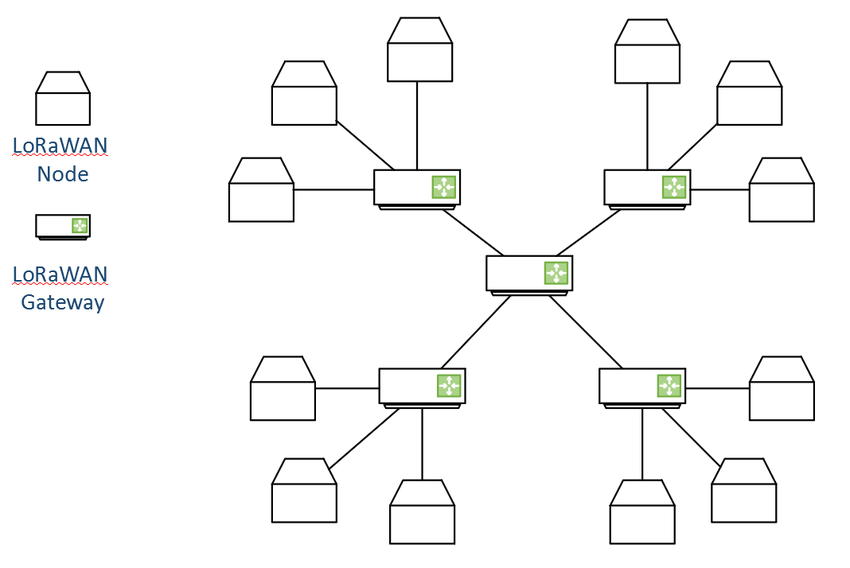
\includegraphics[width=11cm]{stars_topology}
  \caption{Schematisierung einer Star-of-Stars-Netzwerk-Architektur, bestehend aus \textit{Nodes} und \textit{Gateways}, die vom LoRaWAN-Standard verwendet wird\cite{phdthesisLoRA}}
\end{figure}

In der Silvanet-Architektur von Dryad entsprechen die Nodes den Sensoren, die Waldbrände erkennen sollen. Wir nennen sie Sensors.
Silvanet verwendet dann 2 Arten von Gateways, um die Informationen von den Sensoren nach außerhalb des Netzwerks zu leiten (Dryads Cloud-Backend-Service).
Der erste Typ heißt \textit{Mesh-Gateway} und ermöglicht die Netzwerkabdeckung über große Entfernungen zwischen den Sensoren und andere Mesh-Gateways.
Die zweite Art von Gateways, die \textit{Borders Gateways}, übertragen die Daten der Mesh Gateways nach außerhalb des LoRaWAN-Netzwerks, indem sie mit dem Backend-Service von Dryad kommunizieren.

Nach der Verarbeitung können die verschiedenen Informationen der zu Standorten zusammengefassten Sensoren abgerufen und in der Webanwendung von Dryad angezeigt werden.
Mit dieser Anwendung kann sich ein Benutzer anmelden, die Installation von Sensoren an einem Standort planen, die verschiedenen gesammelten Daten in Echtzeit verfolgen und die Art einer Waldbrandwarnung im Detail abrufen.

\begin{figure}[h]
  \centering
  \includegraphics[width=12cm]{silvanet_architecture}
  \caption{Schematische Darstellung des LoRaWAN-Netzwerks, das die verschiedenen Sensoren mit dem Cloud-System verbindet.}
\end{figure}


\begin{figure}[h]
  \centering
  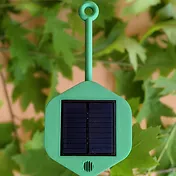
\includegraphics[width=4cm]{dryad_sensor}
  \caption{ein luftschnüffelnder Sensor, der ein Silvanet-Netzwerk bildet}
\end{figure}
